\documentclass{fp-slides}
% \ifx\pdfoutput\undefined
% % we are running LaTeX, not pdflatex
% \usepackage{graphicx}
% \else
% % we are running pdflatex, so convert .eps files to .pdf
% \usepackage[pdftex]{graphicx}
% \usepackage{epstopdf}
% \fi 
\usepackage{graphics}
\newtheorem{defin}{Definition}
\begin{document}

%%%%%%%%%%%%%%% Define code blocks

% \defverbatim[colored]\factCcode{%
% \begin{lstlisting}[frame=single,language=C]
%   int fact(int n)
%   { int x = 1;
%     while (n > 0)
%      { x = x * n;
%        n = n - 1;
%      }
%     return x;
%   }
% \end{lstlisting}}
% 
% \defverbatim[colored]\factMLcode{%
% \begin{lstlisting}[frame=single]
%   let rec fact n =
%     if n = 0 then 1
%     else n * fact(n - 1);;
% \end{lstlisting}}
% 
% \defverbatim[colored]\badFuncCode{%
% \begin{lstlisting}[frame=single]
%   int rand(void)
%   { static int n = 0;
%     return n = 2147001325 * n + 715136305;
%   }
% \end{lstlisting}}

%%%%%%%%%%%%%%%%%%%%%%

\frame{\titlepage}
\frame{
  \frametitle{Formal Logic}
\begin{itemize}
 \item  \Large Propositional calculus
\item Logical functions, Truth Tables
\item Inference rules. Modus Ponens
\end{itemize}


}

\frame{
  \frametitle{Propositional Logic}
\begin{itemize}
 \item \Large Proposition: statement that is either true or false.
\end{itemize}


}
\frame{
  \frametitle{Propositional Logic}
\begin{itemize}
 \item \Large Proposition: statement that is either true or false.
\item \Huge ``This statement is false.''
\end{itemize}

}
\frame{
  \frametitle{Propositional language}
\begin{itemize}
 \item \Large An infinite set of variables(\textbf{propositions})
\item A set of \textbf{operators}
\item Separate values \textbf{TRUE} and \textbf{FALSE}
\end{itemize}

}
\frame{
  \frametitle{Propositional Operators}
\begin{itemize}
 \item \Large  Negation
\item Disjunction
\item Conjunction
\item Implication
\item Equivalence
\end{itemize}


}
\frame{
  \frametitle{Negation}
\Huge
\begin{center}
\begin{tabular}{l|l}

A & $\neg A$\\
TRUE & FALSE\\
FALSE & TRUE
\end{tabular}

\end{center}


}
\frame{
  \frametitle{Disjunction (or)}
\Huge

\begin{center}
\begin{tabular}{l|l|l|l}
$A\vee B$& \textbf{TRUE} & \textbf{FALSE} & \textbf{B}\\ \hline
\textbf{TRUE} & TRUE & TRUE\\  \hline
\textbf{FALSE} & TRUE & FALSE \\ \hline
\textbf{A} 
\end{tabular}
\end{center}


}

\frame{
  \frametitle{Conjunction (and)}
\Huge

\begin{center}
\begin{tabular}{l|l|l}
$A\wedge B$& \textbf{TRUE} & \textbf{FALSE} \\ \hline
\textbf{TRUE} & TRUE & FALSE\\ \hline
\textbf{FALSE} & FALSE & FALSE
\end{tabular}
\end{center}


}

\frame{
  \frametitle{Implication (if$\dots$then)}
\Huge

\begin{center}
\begin{tabular}{l|l|l}
$A\Rightarrow B$ & \textbf{TRUE} & \textbf{FALSE} \\ \hline
\textbf{TRUE} & TRUE & FALSE\\ \hline
\textbf{FALSE} & TRUE & TRUE
\end{tabular}
\end{center}


}

\frame{
  \frametitle{Equivalence}
\Huge

\begin{center}
\begin{tabular}{l|l|l}
$A\Leftrightarrow B$ & \textbf{TRUE} & \textbf{FALSE} \\ \hline
\textbf{TRUE} & TRUE & FALSE\\ \hline
\textbf{FALSE} & FALSE & TRUE
\end{tabular}
\end{center}


}
\frame{
  \frametitle{Inference: Modus Ponens}
\Large Modus Ponens (rule of detachment):


\begin{center}
\begin{tabular}{l|l}
A & Ted is cold\\
$A\Rightarrow B$ & If Ted is cold, he shivers\\ \hline
B & Ted shivers
\end{tabular}
\end{center}


}


\frame{
  \frametitle{Expert and decision support systems in medicine}

  \begin{itemize}
  \item \Large Decision making
    \maybepause
    
  \item \Large Conditional probability
    \maybepause
   \item Expert systems
     \maybepause
   
  \item Clinical Decision-Support Systems
    \maybepause

  
  \end{itemize}
}
% Topic 11 Clinical Decision-Support Systems. Predictive Tools for Clinical Decision Support. .Modeling for Decision Support. Expert systems. 
% History of Systems. Types of Systems. Definition of Clinical Decision-Support Systems. Influence of Decision-Support Systems. Categories of Systems. 
% Development of Predictive Tools. Decision Support with Simple Predictive Tools. Evaluation and Conclusions. 
% A Broad View of Decision Support and Expert Systems. The Knowledge-Level Hypothesis. Knowledge Acquisition and Design Structuring. Modern Architectures for Decision Support.
\frame{
  \frametitle{Decision making}
\textbf{Decision making} -- the processes resulting in the selection of a course of action among several alternatives. Every decision making process produces a final choice. The output can be an action or an opinion of choice.
\begin{enumerate}
 \item Objectives must first be established
 \item Objectives must be classified and placed in order of importance
 \item Alternative actions must be developed
 \item The alternative must be evaluated against all the objectives
 \item The alternative that is able to achieve all the objectives is the tentative decision
 \item The tentative decision is evaluated for more possible consequences
 \item The decisive actions are taken, and additional actions are taken to prevent any adverse consequences from becoming problems 
\end{enumerate}

}
% \frame{
%   \frametitle{Decision making}
% 
% }
\frame{
  \frametitle{Decision support systems}
\textbf{Decision support system} (DSS) is a computer-based information system that supports business or organizational decision-making activities. DSSs serve the management, operations, and planning levels of an organization and help to make decisions, which may be rapidly changing and not easily specified in advance.

\begin{enumerate}
\item A communication-driven DSS supports more than one person working on a shared task
\item A data-driven DSS or data-oriented DSS emphasizes access to and manipulation of a time series of internal company data and, sometimes, external data.
\item A document-driven DSS manages, retrieves, and manipulates unstructured information in a variety of electronic formats.
\item A knowledge-driven DSS provides specialized problem-solving expertise stored as facts, rules, procedures, or in similar structures.
\item A model-driven DSS emphasizes access to and manipulation of a statistical, financial, optimization, or simulation model. 
% Model-driven DSS use data and parameters provided by users to assist decision makers in analyzing a situation; they are not necessarily data-intensive. 
\end{enumerate}

}

% \begin{frame}\frametitle{Conditional probability}
% \begin{itemize}
% \item Let $B$ be an event so that $P(B) > 0$
% \item Then the conditional probability of an event $A$ given that $B$
%   has occurred is
%   $$
%   P(A ~|~ B) = \frac{P(A \cap B)}{P(B)}
%   $$
% % \item Notice that if $A$ and $B$ are independent, then
% %   $$
% %   P(A ~|~ B) = \frac{P(A) P(B)}{P(B)} = P(A)
% %   $$
% \end{itemize}
% \end{frame}
% 
% \begin{frame}\frametitle{Example}
% \begin{itemize}
% \item Consider our die roll example
% \item $B = \{1, 3, 5\}$
% \item $A = \{1\}$
%   \begin{eqnarray*}
% P(\mbox{one given that roll is odd})  & = & P(A ~|~ B) \\ \\
%   & = & \frac{P(A \cap B)}{P(B)} \\ \\
%   & = & \frac{P(A)}{P(B)} \\ \\ 
%   & = & \frac{1/6}{3/6} = \frac{1}{3}
%   \end{eqnarray*}
% \end{itemize}
% \end{frame}

\frame{
  \frametitle{Decision tree}
\textbf{Decision tree} is a decision support tool that uses a tree graph  model of decisions and their possible consequences, including chance event outcomes, resource costs, and utility

\vspace{5mm}
A decision Tree consists of 3 types of nodes:
\begin{enumerate}
\item Decision nodes - commonly represented by squares
\item Chance nodes - represented by circles
\item End nodes - represented by triangles\end{enumerate}
% 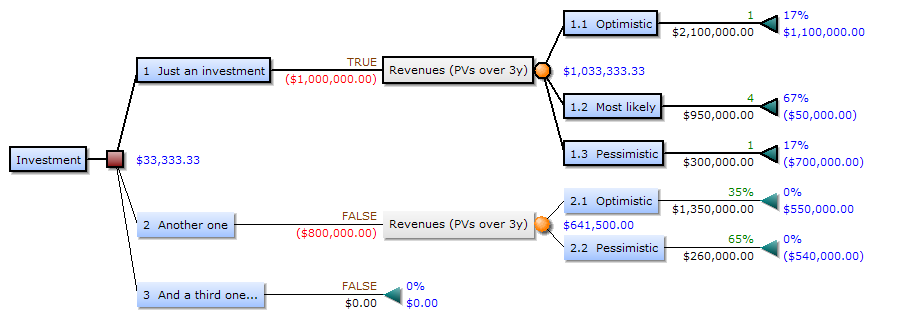
\includegraphics[scale=0.1]{dt}
}
% \frame{
%   \frametitle{Decision tree}
% 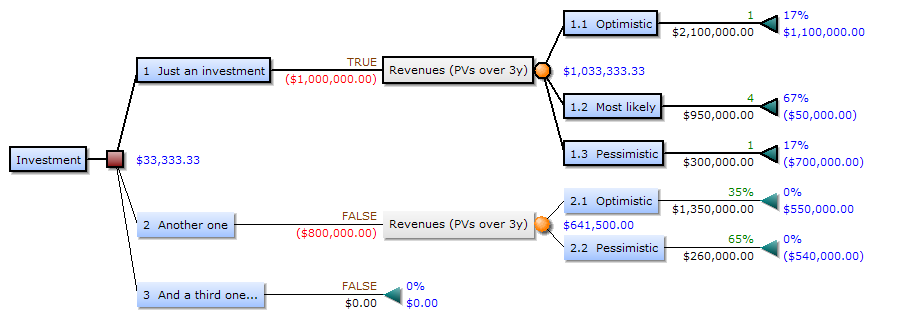
\includegraphics[scale=0.35]{dt}
% }
\frame{
  \frametitle{Knee Surgery -- Decision tree}
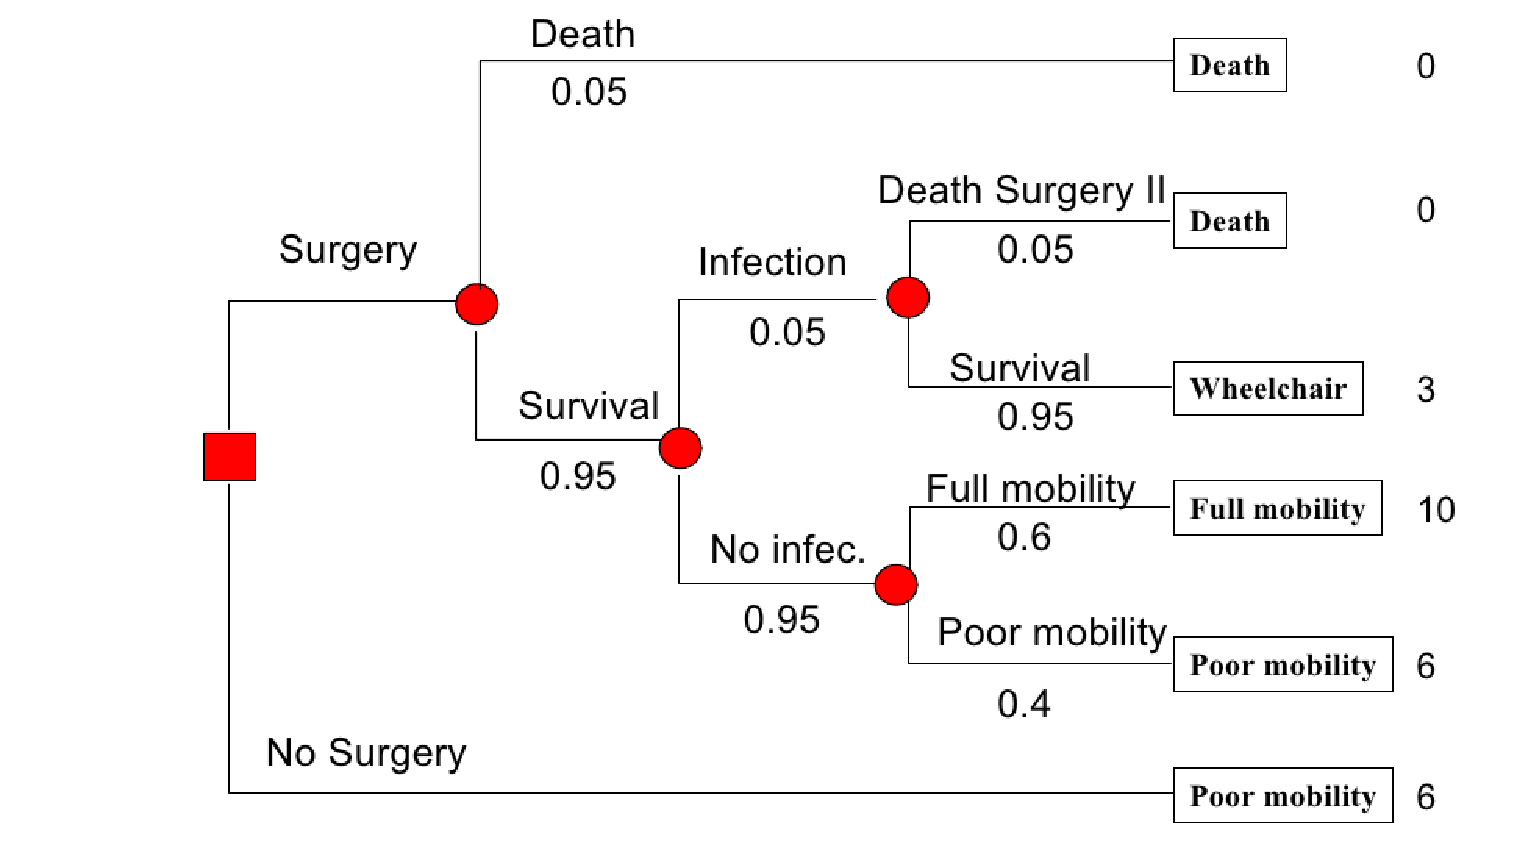
\includegraphics[scale=0.4]{k1}
}
\frame{
  \frametitle{Knee Surgery -- Decision tree}
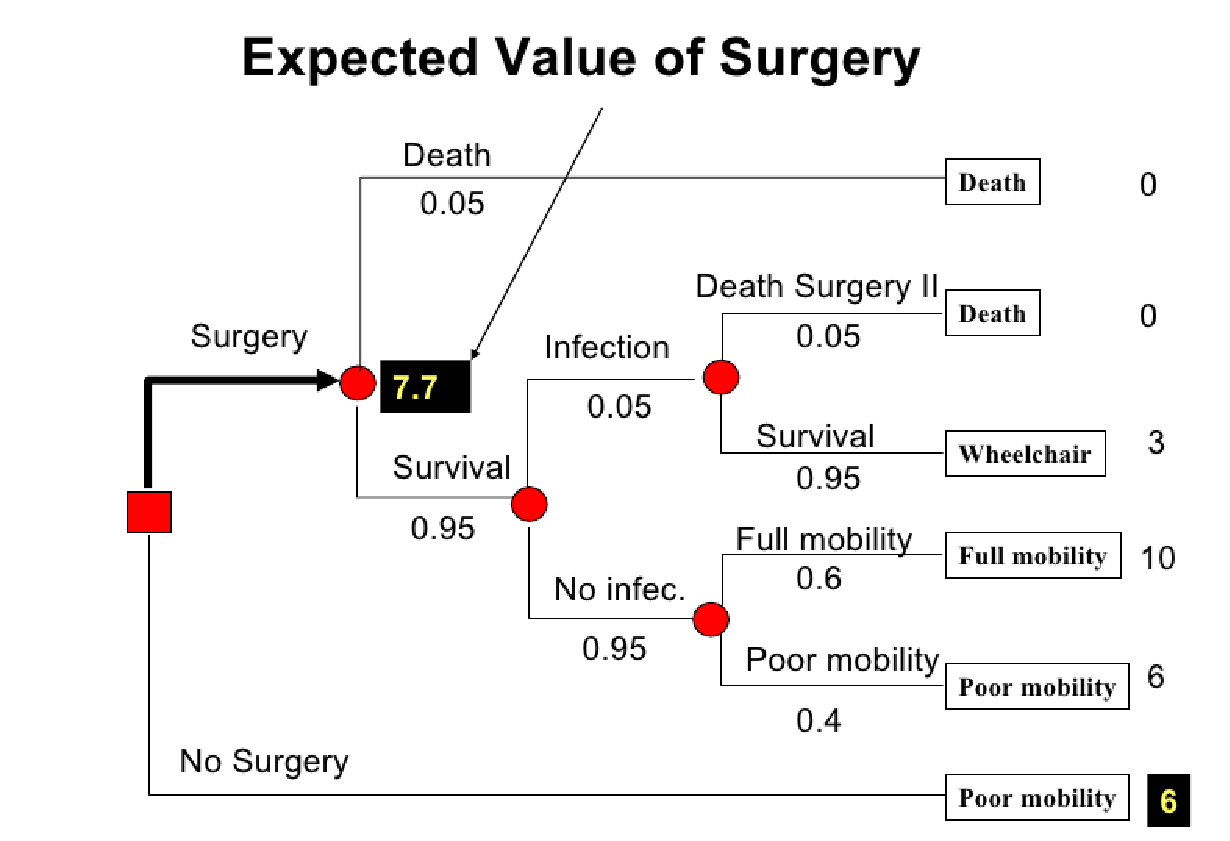
\includegraphics[scale=0.5]{k2}
}
\frame{
  \frametitle{Expert systems}
\textbf{Expert} is a person with extensive knowledge or ability based on research, experience, or occupation and in a particular area of study.

\vspace{5mm}
An \textbf{expert system} is software that uses a knowledge base of human expertise for problem solving, or clarify uncertainties where malmally one or more human experts would need to be consulted. 

\vspace{5mm}
Expert systems are designed to facilitate tasks in the fields of accounting, medicine, process control, financial service, production, human resources, among others. 
% Typically expert systems do not typically provide a definitive answer, but provide probabilistic recommendations.
}
\frame{
  \frametitle{Horn clause}
\textbf{Horn clause} is a clause (a disjunction of literals) with at most one positive literal
\[
(p_1\wedge p_2 \wedge .. \wedge p_n) \to H
 \]


In plain English:
\begin{center}
If ALL conditions  $p_1, p_2, .. ,p_n$ are true, then we can make a conclusion, that a hypothesis H is true
\end{center}

Example:
\vspace{3mm}


$p_1 =$ Cessation of breathing, 
$p_2 =$ No pulse,
$p_3 =$ Pallor mortis,
$p_4 =$ Livor mortis,
$p_5 =$ Algor mortis,
$p_6 =$ Rigor mortis,
$p_7 =$ Decomposition

\vspace{3mm}
Horn clause: $(p_1\wedge p_2 \wedge .. \wedge p_7) \to$ patient is dead
}
\frame{
  \frametitle{Expert systems - Certainty factors}
 Typically, the problem area is complex enough that a more simple traditional algorithm cannot provide a proper solution. As such, expert systems do not typically provide a definitive answer, but provide probabilistic recommendations.


\vspace{3mm}
The rule-based expert system introduced a quasi-probabilistic approach called \textbf{certainty factors}


\vspace{3mm}
The \textbf{certainty factor} is a number that quantify uncertainty in the degree to which the available evidence supports a hypothesis.


\vspace{3mm}
CF are used to reflect the fact, that human, when reasoning, does not always make statements with 100\% confidence.

If patiant is decompositiong, then he is probably dead.


}
\frame{
  \frametitle{Expert systems - Chaining}
Two methods of reasoning when using inference rules are forward chaining and backward chaining.


\vspace{3mm}
\textbf{Forward chaining} starts with the data available and uses the inference rules to extract more data until a desired goal is reached. 

\vspace{2mm}
\scriptsize
An inference engine using forward chaining searches the inference rules until it finds one in which the if clause is known to be true. It then concludes the then clause and adds this information to its data. It continues to do this until a goal is reached. Because the data available determines which inference rules are used, this method is also classified as data driven.

\normalsize
\vspace{3mm}
\textbf{Backward chaining }starts with a list of goals and works backwards to see if there is data which will allow it to conclude any of these goals. 

\vspace{2mm}
\scriptsize
An inference engine using backward chaining would search the inference rules until it finds one which has a then clause that matches a desired goal. If the if clause of that inference rule is not known to be true, then it is added to the list of goals. 
}

\frame{
  \frametitle{Expert systems - Chaining}
\begin{enumerate}
\item IF X is green THEN X is a frog. (Confidence Factor: +1\%)
\item IF X is NOT green THEN X is NOT a frog. (Confidence Factor: +99\%)
\item IF X is a frog THEN X hops. (Confidence Factor: +50\%)
\item IF X is NOT a frog THEN X does NOT hop. (Confidence Factor +50\%)
\end{enumerate}


Suppose a goal is to conclude that Fritz hops. Let X = "Fritz".


}
% \frame{
%   \frametitle{Expert systems - Chaining}
% The goal is to conclude that Fritz hops. 
% 
%  The rule base would be searched and rule (3) would be selected because its conclusion (the then clause) matches the goal. It is not known that Fritz is a frog, so this "if" statement is added to the goal list. The rule base is again searched and this time rule (1) is selected because its then clause matches the new goal just added to the list. This time, the if clause (Fritz is green) is known to be true and the goal that Fritz hops is concluded. Because the list of goals determines which rules are selected and used, this method is called goal driven.
% 
% }
\frame{
  \frametitle{Clinical Decision Support Systems}
\textbf{Clinical Decision Support systems} link health observations with health knowledge to influence health choices by clinicians for improved health care.

Most CDSS consist of three parts:
\begin{enumerate}
\item  the knowledge base, 
\item  inference engine
\item  mechanism to communicate. (Human-Computer Interface)
\end{enumerate}
}
\frame{
  \frametitle{Effectiveness of CDSS}
A systematic reviews  of CDSs usage in healtcare concluded that CDSs improved practitioner performance in \textbf{64-68\%} of the trials. The CDSs improved patient outcomes in \textbf{13\% }of the trials. 

\vspace{3mm}
The CDSs features associated with success include the following:
\begin{enumerate}
\item the CDSs is integrated into the clinical workflow rather than as a separate log-in or screen.
\item the CDSs is electronic rather than paper-based templates.
\item the CDSs provides decision support at the time and location of care rather than prior to or after the patient encounter.
\item the CDSs provides recommendations for care, not just assessments.                                                                                \end{enumerate}

}
\frame{
\frametitle{Dixi}

\begin{center}
\Huge Dixi\end{center}
}
\end{document}
